%%
%% This is file `./samples/longsample.tex',
%% generated with the docstrip utility.
%%
%% The original source files were:
%%
%% apa7.dtx  (with options: `longsample')
%% ----------------------------------------------------------------------
%% 
%% apa7 - A LaTeX class for formatting documents in compliance with the
%% American Psychological Association's Publication Manual, 7th edition
%% 
%% Copyright (C) 2021 by Daniel A. Weiss <daniel.weiss.led at gmail.com>
%% 
%% This work may be distributed and/or modified under the
%% conditions of the LaTeX Project Public License (LPPL), either
%% version 1.3c of this license or (at your option) any later
%% version.  The latest version of this license is in the file:
%% 
%% http://www.latex-project.org/lppl.txt
%% 
%% Users may freely modify these files without permission, as long as the
%% copyright line and this statement are maintained intact.
%% 
%% This work is not endorsed by, affiliated with, or probably even known
%% by, the American Psychological Association.
%% 
%% ----------------------------------------------------------------------
%% 
\documentclass[man]{apa7}

\usepackage{lipsum}

\usepackage[american]{babel}

\usepackage{caption} % For captioning outside figures
\usepackage{capt-of} % For captioning outside figures

\usepackage{csquotes}
\usepackage[style=apa,backend=biber]{biblatex}
\addbibresource{bibliography.bib}

\title{Laser Scanning Comparison Using CloudCompare}
\shorttitle{}

\authorsnames{Jule Valendo Halim -1425567}
\authorsaffiliations{GEOM90038 - Advanced Imaging}

\begin{document}
\maketitle
\section{Introduction}


\Textcite{Jones2022} said this

\section{Method}

\subsection{Procedure}


\section{Results}
Table~\ref{tab:BasicTable} summarizes the data. \lipsum[1-3]
\vspace{20pt}

\begin{minipage}{\linewidth}
  \captionof{table}{Sample Basic Table}
  \label{tab:BasicTable}
  \begin{tabular}{@{}llr@{}}         \toprule
  \multicolumn{2}{c}{Item}        \\ \cmidrule(r){1-2}
  Animal    & Description & Price \\ \midrule
  Gnat      & per gram    & 13.65 \\
            & each        &  0.01 \\
  Gnu       & stuffed     & 92.50 \\
  Emu       & stuffed     & 33.33 \\
  Armadillo & frozen      &  8.99 \\ \bottomrule
  \end{tabular}
\end{minipage}

\vspace{20pt}

\lipsum[1]

Figure~\ref{fig:Figure1} shows this trend.

\vspace{20pt}
\begin{minipage}{\linewidth}
  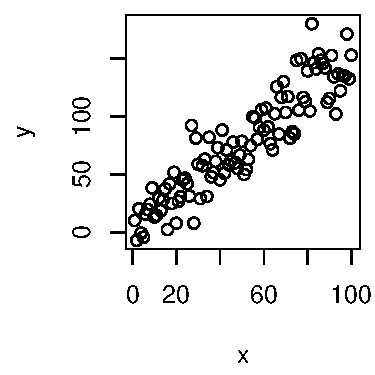
\includegraphics[bb=0in 0in 2.5in 2.5in, height=2.5in, width=2.5in]{figures/Figure1.pdf}
  \captionof{figure}{This is my first figure caption.}
  \label{fig:Figure1}
\end{minipage}

\section{Discussion}
\lipsum[17]

\lipsum[18]

\lipsum[19]

\printbibliography


\end{document}

%% 
%% Copyright (C) 2021 by Daniel A. Weiss <daniel.weiss.led at gmail.com>
%% 
%% This work may be distributed and/or modified under the
%% conditions of the LaTeX Project Public License (LPPL), either
%% version 1.3c of this license or (at your option) any later
%% version.  The latest version of this license is in the file:
%% 
%% http://www.latex-project.org/lppl.txt
%% 
%% Users may freely modify these files without permission, as long as the
%% copyright line and this statement are maintained intact.
%% 
%% This work is not endorsed by, affiliated with, or probably even known
%% by, the American Psychological Association.
%% 
%% 
%% This work is "maintained" (as per LPPL maintenance status) by
%% Daniel A. Weiss.
%% 
%% This work consists of the file  apa7.dtx
%% and the derived files           apa7.ins,
%%                                 apa7.cls,
%%                                 apa7.pdf,
%%                                 README,
%%                                 APA7american.txt,
%%                                 APA7british.txt,
%%                                 APA7dutch.txt,
%%                                 APA7english.txt,
%%                                 APA7french.txt,
%%                                 APA7german.txt,
%%                                 APA7ngerman.txt,
%%                                 APA7greek.txt,
%%                                 APA7czech.txt,
%%                                 APA7turkish.txt,
%%                                 APA7endfloat.cfg,
%%                                 Figure1.pdf,
%%                                 shortsample.tex,
%%                                 longsample.tex, and
%%                                 bibliography.bib.
%% 
%%
%% End of file `./samples/longsample.tex'.
